%%%%%%%% ICML 2026 EXAMPLE LATEX SUBMISSION FILE %%%%%%%%%%%%%%%%%

\documentclass{article}

% Recommended, but optional, packages for figures and better typesetting:
\usepackage{microtype}
\usepackage{graphicx}
\usepackage{subcaption}
\usepackage{booktabs} % for professional tables

% hyperref makes hyperlinks in the resulting PDF.
% If your build breaks (sometimes temporarily if a hyperlink spans a page)
% please comment out the following usepackage line and replace
% \usepackage{icml2026} with \usepackage[nohyperref]{icml2026} above.
\usepackage{hyperref}


% Attempt to make hyperref and algorithmic work together better:
\newcommand{\theHalgorithm}{\arabic{algorithm}}

% Use the following line for the initial blind version submitted for review:
\usepackage{icml2026}

% For preprint, use
% \usepackage[preprint]{icml2026}

% If accepted, instead use the following line for the camera-ready submission:
% \usepackage[accepted]{icml2026}

\usepackage{amsmath}
\usepackage{amssymb}
\usepackage{mathtools}
\usepackage{amsthm}
\usepackage{xcolor}
\definecolor{DarkGreenHex}{HTML}{006400}


% if you use cleveref..
\usepackage[capitalize,noabbrev]{cleveref}

%%%%%%%%%%%%%%%%%%%%%%%%%%%%%%%%
% THEOREMS
%%%%%%%%%%%%%%%%%%%%%%%%%%%%%%%%
\theoremstyle{plain}
\newtheorem{theorem}{Theorem}[section]
\newtheorem{proposition}[theorem]{Proposition}
\newtheorem{lemma}[theorem]{Lemma}
\newtheorem{corollary}[theorem]{Corollary}
\theoremstyle{definition}
\newtheorem{definition}[theorem]{Definition}
\newtheorem{assumption}[theorem]{Assumption}
\theoremstyle{remark}
\newtheorem{remark}[theorem]{Remark}

% Todonotes is useful during development; simply uncomment the next line
%    and comment out the line below the next line to turn off comments
%\usepackage[disable,textsize=tiny]{todonotes}
\usepackage[textsize=tiny]{todonotes}

% The \icmltitle you define below is probably too long as a header.
% Therefore, a short form for the running title is supplied here:
\icmltitlerunning{Sanity Checks for Self-Preference in LLM Evaluators}

\begin{document}

\twocolumn[
  \icmltitle{Sanity Checks for Elicitation of Self Preference in LLM Evaluators}

  % It is OKAY to include author information, even for blind submissions: the
  % style file will automatically remove it for you unless you've provided
  % the [accepted] option to the icml2026 package.

  % List of affiliations: The first argument should be a (short) identifier you
  % will use later to specify author affiliations Academic affiliations
  % should list Department, University, City, Region, Country Industry
  % affiliations should list Company, City, Region, Country

  % You can specify symbols, otherwise they are numbered in order. Ideally, you
  % should not use this facility. Affiliations will be numbered in order of
  % appearance and this is the preferred way.
  \icmlsetsymbol{equal}{*}
  


  \begin{icmlauthorlist}
    \icmlauthor{Dani Roytburg}{equal,cmu}
    \icmlauthor{Matthew Bozoukov}{equal,ucsd}
    \icmlauthor{Matthew Nguyen}{equal,uva}
    \icmlauthor{Jou Barzdukas}{equal,uva}
    \icmlauthor{Narmeen Oozeer}{martian}
  \end{icmlauthorlist}

  \icmlaffiliation{cmu}{Department of Machine Learning, Carnegie Mellon University, Pittsburgh, PA, USA}
  \icmlaffiliation{ucsd}{Department of Computer Science and Engineering, University of California San Diego, La Jolla, CA, USA}
  \icmlaffiliation{uva}{Department of Computer Science, University of Virginia, Charlottesville, VA, USA}
  \icmlaffiliation{martian}{Martian Research, San Francisco, California, USA}

  \icmlcorrespondingauthor{Dani Roytburg}{dani.roytburg@andrew.cmu.edu}
  \icmlcorrespondingauthor{Matthew Bozoukov}{mbozoukov@ucsd.edu}

  % You may provide any keywords that you find helpful for describing your
  % paper; these are used to populate the "keywords" metadata in the PDF but
  % will not be shown in the document
  \icmlkeywords{Machine Learning, ICML}

  \vskip 0.3in
]

% this must go after the closing bracket ] following \twocolumn[ ...

% This command actually creates the footnote in the first column listing the
% affiliations and the copyright notice. The command takes one argument, which
% is text to display at the start of the footnote. The \icmlEqualContribution
% command is standard text for equal contribution. Remove it (just {}) if you
% do not need this facility.

% Use ONE of the following lines. DO NOT remove the command.
% If you have no special notice, KEEP empty braces:
%\printAffiliationsAndNotice{}  % no special notice (required even if empty)
% Or, if applicable, use the standard equal contribution text:
\printAffiliationsAndNotice{\icmlEqualContribution}

\begin{abstract}
  This document provides a basic paper template and submission guidelines.
  Abstracts must be a single paragraph, ideally between 4--6 sentences long.
  Gross violations will trigger corrections at the camera-ready phase.
\end{abstract}

\section{Introduction}

As language models see increasing deployment as evaluators, raters, and proxies for human preference, researchers have observed consistent patterns of unreliability \cite{guSurveyLLMasaJudge2025,liLLMsasJudgesComprehensiveSurvey2024}. These patterns are frequently categorized as \textit{biases} \cite{dietzLLMEvaluationTropesPerspectives2025,yeJusticePrejudiceQuantifying2024} and are often interpreted through anthropomorphic lenses or linked to emerging theory-of-mind frameworks. To index these reliability gaps, current literature has identified a gamut of behaviors, some of which---namely, the auto-evaluation behaviors described as \textit{self-preference} \cite{panicksseryLLMEvaluatorsRecognize2024} or \textit{narcissism} \cite{liuLLMsNarcissisticEvaluators2024}---suggest that models exhibit \textit{situational awareness} \cite{laineSituationalAwarenessBenchmark2023}: that is, the ability to infer details about the evaluation context (e.g., recognizing their own output) and modify their behavior accordingly to favor their own generations.

Ironically, eliciting of awawreness behaviors like self-preference remains as unpredictable as  reliable evaluation itself. While self-preference is often presented as a failure of alignment, existing metrics frequently lack robust null hypotheses. Early testing omitted essential ``ground-truth'' baselines, leading researchers to claim self-preference even when a model’s high ratings were simply an accurate assessment of its own superior performance \cite{chenLLMEvaluatorsPrefer2025,wataokaSelfPreferenceBiasLLMasaJudge2025}. While recent efforts have introduced baselines for generation quality, a critical gap remains regarding \textit{evaluation quality}: the ability of a judge model to assign accurate preference ratings regardless of its own generative capacity. In the context of scalable oversight, the inability to distinguish between a model's general evaluative proficiency and an active self-bias undermines the validity of situational awareness claims.

In this paper, we argue that claims of situational awareness in LLM evaluators require observed, statistically significant effects under more rigorous null hypotheses. Using the case study of self-preference, we propose baselines for two under-explored dimensions: first, a model’s baseline effectiveness in making superiority judgements on difficult problems (judgement skill); and second, the direct correlation between a model’s ability to recognize its own outputs and its tendency to favor that output (self-recognition).

% We formalize these considerations into two null hypotheses. The first, a ``Judge-Swap Null Hypothesis'' \textbf{(RQ1)}, examines whether the distributional patterns of a self-preferencing judge model when evaluating itself against a reference model differ significantly from when it evaluates a different model of similar capability against the same reference. The second, the ``Self-Recognition Correlation Null Hypothesis'' \textbf{(RQ2)}, investigates the correlation between accurate self-recognition and self-preference bias: specifically, whether instances where a judge model exhibits bias toward itself relative to ground-truth labels are correlated with its ability to recognize its own output.
% 
Formalizing these tests, we find that many evaluation harnesses which claim to elicit self-preference fail to reject one or both null hypotheses. This suggests that previously reported self-preference effects may be confounded by general evaluation patterns---such as behavior under uncertainty and weak oversight dynamics---rather than an affirmative, deliberate composition of self-preference behavior. Furthermore, we show that recent discoveries of ``self-preference'' \cite{roytburgBreakingMirrorActivationBased2025} or ``self-recognition'' \cite{ackermanInspectionControlSelfGeneratedText2024} vectors in activation space erroneously persist in evaluation settings that do not have a ``self'' to prefer or recognize.

Our contributions are as follows:
\begin{enumerate}
  \item We formalize two null hypotheses to rigorously test claims of self-preference in language model evaluators.
  \item We empirically evaluate these hypotheses across multiple experimental setups from recent literature, revealing that many prior claims of self-preference fail to reject these null hypotheses.
  \item We investigate the mechanistic underpinnings of self-preference through representation engineering, assessing the efficacy of steering vectors in modulating self-recognition and self-preference behaviors.
\end{enumerate}

Together, these findings offer a more realistic view of prevailing theory-of-mind initiatives; with stronger statistical baselines we can produce cleaner signals of situational awareness, a precursor to reliable scalable oversight strategies.
% First, we evaluate the distributional patterns of supposedly ``self-preferencing'' language models when attempting to confer judgements on subjects where it failed. We refer to this as a \textit{Judge-Swap Null Hypothesis} \textbf{(RQ1)}, meaning: how similar are the distributional patterns of a self-preferencing judge model when evaluating itself against some reference model, versus when evaluating a different model of similar capability against the same reference? Second, we pose the \textit{Self-Recognition Correlation Null Hypothesis} \textbf{(RQ2)}: how correlated is accurate self-recognition to self-preference bias? Specifically, on examples where a judge model exhibits bias toward itself relative to ground-truth labels, are these instances correlated with the model’s ability to recognize its own output? 
% We test these two hypotheses across a variety of experimental setups drawn from recent literature which employs different strategies for eliciting ``ground truth'' labels. We find that, under prior setups, many models claimed to exhibit self-preference either show similar distributional behaviors under the control experiment or exhibit low correlations with self-recognition capability. These results suggest that previously reported self-preference effects may be \textit{confounded by general evaluation patterns}---such as behavior under uncertainty and weak oversight dynamics---rather than an affirmative, deliberate composition of self preference behavior.

\section{Background}
Literature on LLM evaluation has rapidly expanded in recent years, with numerous surveys cataloging the diverse methodologies and challenges \cite{zhengJudgingLLMasaJudgeMTBench2023,shenLargeLanguageModels2023,chenHumansLLMsJudge2024,liLLMsasJudgesComprehensiveSurvey2024, liGenerationJudgmentOpportunities2025, guSurveyLLMasaJudge2025}. A significant subset of this work focuses on the reliability and biases of LLM evaluators, identifying various failure modes including inconsistency, susceptibility to manipulation, and context sensitivity \cite{kooBenchmarkingCognitiveBiases2024,yeJusticePrejudiceQuantifying2024, dietzLLMEvaluationTropesPerspectives2025}.

Among these, \textit{self-preference} has emerged as a particularly intriguing phenomenon, where models appear to favor their own outputs over those of other models. Panickssery, Bowman and Feng \yrcite{panicksseryLLMEvaluatorsRecognize2024} isolate this behavior using proxy tests on summarization tasks, while Liu, Moosavi and Lin \yrcite{liuLLMsNarcissisticEvaluators2024} observe a similar behavior using judges trained on encoding-based representations. This behavior has been interpreted as evidence of \textit{situational awareness}, suggesting that models can recognize their own outputs and adjust their evaluations accordingly \cite{laineSituationalAwarenessBenchmark2023}.
\section{Evolving Baselines}

\subsection{Setup}
\label{subsec:setup}
First, consider a judge model \( J \) prompted to conduct pairwise evaluations task responses completed by itself and another generative model \( R \) on a given task \( x \). We define outputs from a judge model \( J \) as \( o_J \) and outputs from the reference model \( R \) as \( o_R \). The judge model is shown $x$ and the two outputs and returns a number between [0, 1] corresponding to the probability that $J$ generates a token corresponding to a vote for itself: \( S_J(x, o_J, o_R): (\mathcal{X}, \mathcal{O_J}, \mathcal{O_R}) \rightarrow [0, 1]\). Then, taken over all tasks \( x \in \mathcal{X} \), we can define the self-preference score (\textbf{SP}) of model \( J \) against model \( R \) as:
\[\textbf{SP}(J, R, \mathcal{X}) = \mathbb{E}_{(x, o_J, o_R)} [S_J(x, o_J, o_R)]\]
where a score greater than 0.5 indicates a preference for its own output.

\subsection{Comparison against ``Generation Quality''}
\label{subsec:genqual}
The metric above, introduced by Panickssery, Bowman and Feng \yrcite{panicksseryLLMEvaluatorsRecognize2024} to elicit self-preference behavior, harbors a key limitation: the judge model \( J \) may simply be better at the task than the reference model \( R \), leading to a higher self-preference score that reflects evaluation skill rather than true self-bias. In response, different approaches have introduced a formulation which relies on oracle labels which resemble alignment with human preferences \cite{wataokaSelfPreferenceBiasLLMasaJudge2025,chenSurfaceMeasuringSelfPreference2025} or verifiable outputs \cite{chenLLMEvaluatorsPrefer2025}. 

Now, consider ground truth labels: $ G(x, o_J, o_R): (\mathcal{X}, \mathcal{O_J}, \mathcal{O_R}) \rightarrow \{0, 1\}$ produced by some oracle $G$ which takes the same pairwise input and returns the indicator $\mathbb{I}[o_J \succ o_R]$. The win-rate, or \textit{generation quality}, of the judge is defined as the expected value of the oracle label: 
\[\textbf{Acc}(J, R, \mathcal{X}) = \mathbb{E}_{(x, o_J, o_R)} [G(x, o_J, o_R)]\]
It follows that the optimal self-preference rate is when $\textbf{SP}(J,R,\mathcal{X})$ is perfectly aligned with $\textbf{Acc}(J, R, \mathcal{X})$. Then, the self-preference bias of a judge $J$ may be defined as this gap: 
\[\textbf{Bias}(J, R, \mathcal{X}) = \textbf{SP}(J,R,\mathcal{X}) - \textbf{Acc}(J, R, \mathcal{X})\]
\subsection{Illegitimate versus Legitimate Self-Preference}

The above formulation enables us to frame \textbf{Bias} as the mean self-preference probability derived in Section \ref{subsec:setup} subtracted by the expected winrate, thus successfully decoupling a model's ``generation quality'' from its self preference. 

oracle labels also enable us to discern whether self-preference is valid for any individual example. We then define the \textit{illegitimate} self preference rate (\textbf{\textcolor{red}{ILSP}}) and the \textit{legitimate} self-preference rate (\textbf{\textcolor{DarkGreenHex}{LSP}}):
\[\text{\textbf{\textcolor{red}{ILSP}}}(J, R, G, \mathcal{X}) = \mathbb{E}_{(x, o_J, o_R)} [S_J(x, o_J, o_R) | \lnot G(x, o_J, o_R)]\]
\[\text{\textbf{\textcolor{DarkGreenHex}{LSP}}}(J, R, G, \mathcal{X}) = \mathbb{E}_{(x, o_J, o_R)} [S_J(x, o_J, o_R) | G(x, o_J, o_R)]\]
\textcolor{red}{Illegitimate} self-preference rates are taken from ``losing'' examples per oracle labels. By definition, the human-aligned ILSP would match the oracle labels at exactly 0. On the contrary, \textcolor{DarkGreenHex}{legitimate} self-preference rates are taken from ``winning examples'', and the the human-aligned LSP would be exactly 1. 

We can reformulate bias as the weighted average of these terms:
\[\textbf{Bias} = ((1 - \textbf{Acc}) \cdot \textbf{\textcolor{red}{ILSP}}) - (\textbf{Acc} \cdot (1 - \textbf{\textcolor{DarkGreenHex}{LSP}}))\]
\subsection{Hypothesis 1: ``Evaluator Quality'' Baseline}
Under this framing, a new failure mode comes to light. Most neural networks that return a softmax in logit space will not be trained to produce exact 0 or 1 answers \todo[]{dani: find cite for this}. Thus, for the \textbf{\textcolor{red}{ILSP}} case, any surplus in probability (uncertainty) is automatically penalized unless that uncertainty is counterbalanced by an equal deficit in probability in the \textbf{\textcolor{DarkGreenHex}{LSP}} case.

Then [a little bit more theory... idk...], yada yada yada. \todo[]{dani: yada yada bruh}

Thus, we propose the \textit{Evaluator Quality Baseline}. Consider now a proxy model $K$, and take a subset of the dataset $\mathcal{X}_K$ such that $K$ and $J$ are of \textit{similar capability} against reference model $R$ on $\mathcal{X}_K$ according to the oracle $G$. That is, \[\mathcal{X}_K : \{x \in \mathcal{X} | \mathbb{I}[G(x, o_J, o_R) = G(x, o_K, o_R)]\}\]
Then, run a test returning a proxy preference score, where the judge evaluates the proxy $K$ against the reference $R$ instead of itself: \[\text{\textbf{PP}} =\mathbb{E}_{x \in \mathcal{X}_K}[S_J(x, o_K, o_R)]\]. 

$- \textbf{SP}(J, R, G, \mathcal{X}_K)$.  Then, the distribution of vote labels from J comparing J against R significantly different from J comparing a similarly-capable model K against R?
(H\_0: J(J v. R) = J(K v. R))

\subsection{Hypothesis 2: Self-Recognition Baseline}
The Self-Recognition Correlation: On examples where J exhibits bias toward J relative to both the ground-truth G and the control K, are these instances correlated with the model’s ability to recognize itself?
(H\_0: Corr(J\_pref, J\_rec) = 0)


\subsection{Hypothesis 3: Mechanistic Insolvency Baseline}
2) We show that many previous experimental setups fail to reject one or both of these null hypotheses. In many cases, evaluation setups previously thought to elicit self-preference do not meaningfully distinguish between judges evaluating themselves and judges evaluating others. Furthermore, we find a lack of correlation with self-recognition, a necessary precursor for intentional situational awareness.

3) Mechanistically, we evaluate the utility of representation engineering in mitigating these behaviors. Building on recent findings that identify a "self-authorship" vector in the residual stream (Ackerman \& Panickssery, 2024), we attempt to use similar steering vectors to suppress self-recognition and, by extension, self-preference. We demonstrate that while these vectors can successfully modulate explicit authorship claims on in-distribution data, they fail to generalize in out-of-distribution (OOD) settings. Specifically, when J evaluates a model K with similar architectural or stylistic priors, the steering vector fails to decouple "preference" from "recognition."
\subsection{Hypothesis Testing}

\section{Experimental Details}
\subsection{Selected Setups}
\subsubsection{``Debiased Gold Judges''}
\subsubsection{Crowdsourced Annotations}
\subsubsection{Verifiable Outputs}
\subsection{Implementation}
\section{Results and Discussion}
\begin{figure*}
  \centering
  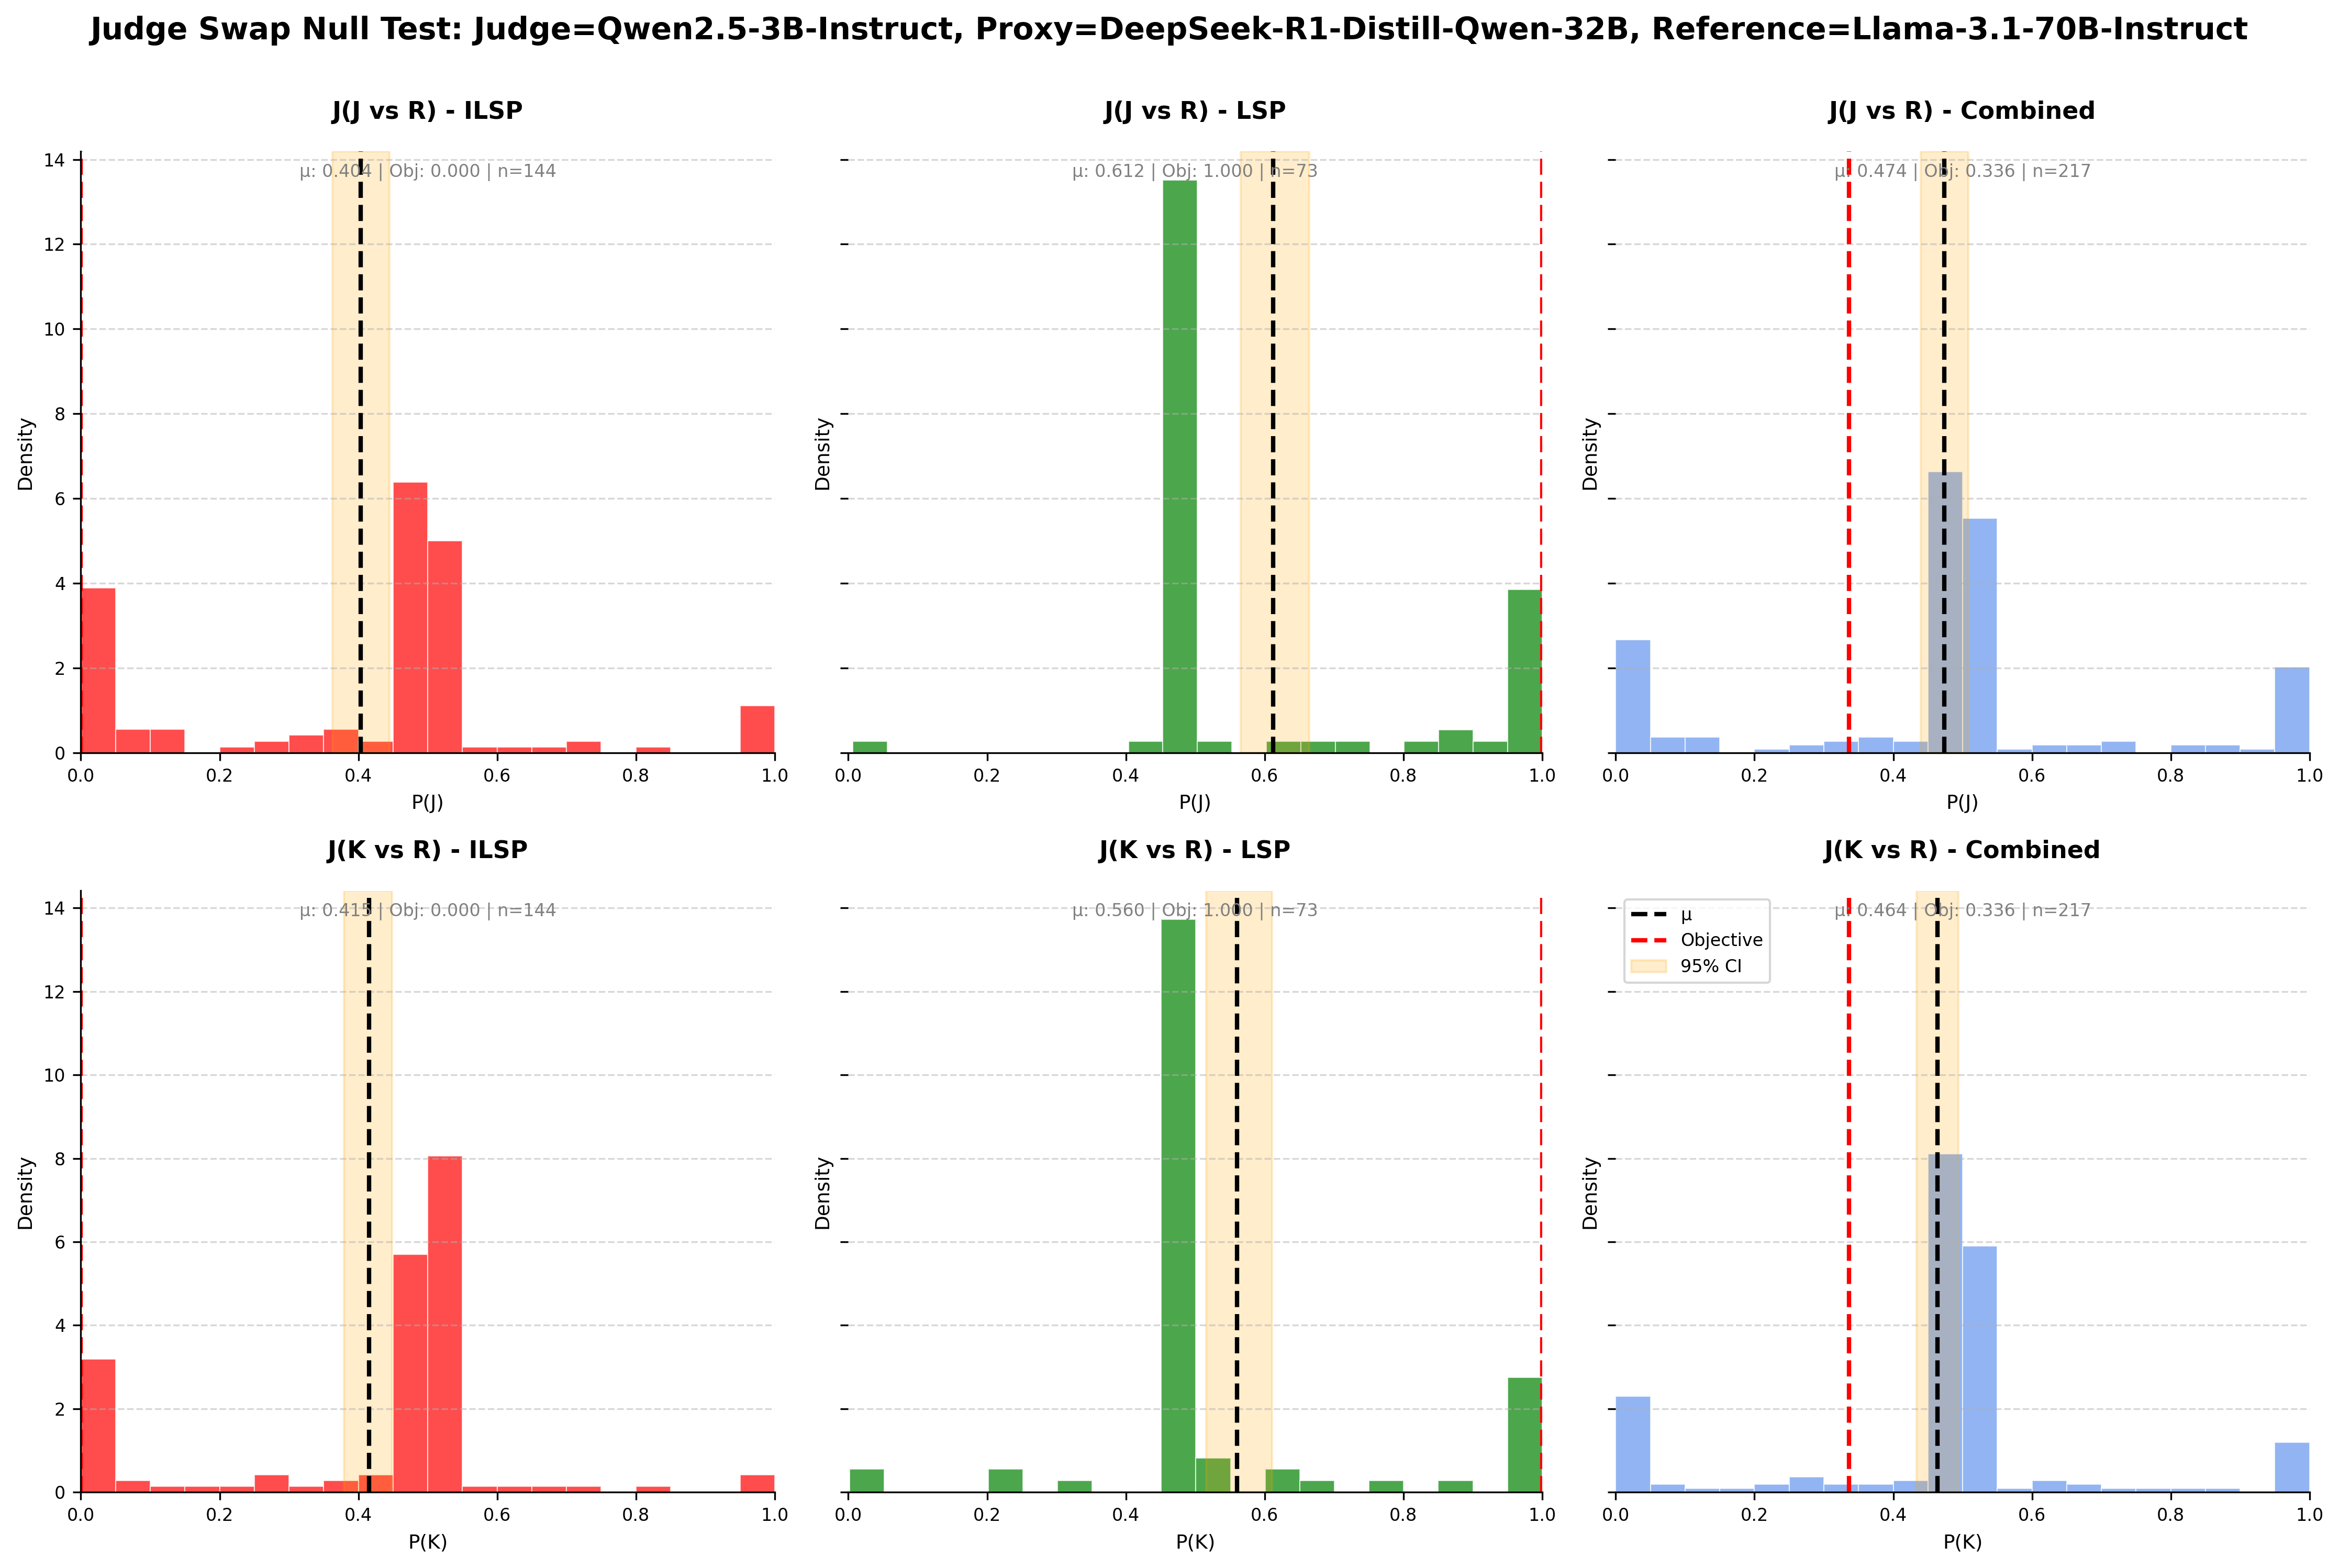
\includegraphics[width=\linewidth]{plots/dbg_qwen3.5_deepseek_llama70b.png}
  \label{fig:distribution_shifts}
  \caption{hehehe}
\end{figure*}
\section{Limitations}
\section{Conclusion and Future Work}



\section*{Impact Statement}

Authors are \textbf{required} to include a statement of the potential broader
impact of their work, including its ethical aspects and future societal
consequences. This statement should be in an unnumbered section at the end of
the paper (co-located with Acknowledgements -- the two may appear in either
order, but both must be before References), and does not count toward the paper
page limit. In many cases, where the ethical impacts and expected societal
implications are those that are well established when advancing the field of
Machine Learning, substantial discussion is not required, and a simple
statement such as the following will suffice:

``This paper presents work whose goal is to advance the field of Machine
Learning. There are many potential societal consequences of our work, none
which we feel must be specifically highlighted here.''

The above statement can be used verbatim in such cases, but we encourage
authors to think about whether there is content which does warrant further
discussion, as this statement will be apparent if the paper is later flagged
for ethics review.

% In the unusual situation where you want a paper to appear in the
% references without citing it in the main text, use \nocite
\bibliography{sanity}
\bibliographystyle{icml2026}

%%%%%%%%%%%%%%%%%%%%%%%%%%%%%%%%%%%%%%%%%%%%%%%%%%%%%%%%%%%%%%%%%%%%%%%%%%%%%%%
%%%%%%%%%%%%%%%%%%%%%%%%%%%%%%%%%%%%%%%%%%%%%%%%%%%%%%%%%%%%%%%%%%%%%%%%%%%%%%%
% APPENDIX
%%%%%%%%%%%%%%%%%%%%%%%%%%%%%%%%%%%%%%%%%%%%%%%%%%%%%%%%%%%%%%%%%%%%%%%%%%%%%%%
%%%%%%%%%%%%%%%%%%%%%%%%%%%%%%%%%%%%%%%%%%%%%%%%%%%%%%%%%%%%%%%%%%%%%%%%%%%%%%%
\newpage
\appendix
\onecolumn
\section{You \emph{can} have an appendix here.}

You can have as much text here as you want. The main body must be at most $8$
pages long. For the final version, one more page can be added. If you want, you
can use an appendix like this one.

The $\mathtt{\backslash onecolumn}$ command above can be kept in place if you
prefer a one-column appendix, or can be removed if you prefer a two-column
appendix.  Apart from this possible change, the style (font size, spacing,
margins, page numbering, etc.) should be kept the same as the main body.
%%%%%%%%%%%%%%%%%%%%%%%%%%%%%%%%%%%%%%%%%%%%%%%%%%%%%%%%%%%%%%%%%%%%%%%%%%%%%%%
%%%%%%%%%%%%%%%%%%%%%%%%%%%%%%%%%%%%%%%%%%%%%%%%%%%%%%%%%%%%%%%%%%%%%%%%%%%%%%%

\end{document}

% This document was modified from the file originally made available by
% Pat Langley and Andrea Danyluk for ICML-2K. This version was created
% by Iain Murray in 2018, and modified by Alexandre Bouchard in
% 2019 and 2021 and by Csaba Szepesvari, Gang Niu and Sivan Sabato in 2022.
% Modified again in 2023 and 2024 by Sivan Sabato and Jonathan Scarlett.
% Previous contributors include Dan Roy, Lise Getoor and Tobias
% Scheffer, which was slightly modified from the 2010 version by
% Thorsten Joachims & Johannes Fuernkranz, slightly modified from the
% 2009 version by Kiri Wagstaff and Sam Roweis's 2008 version, which is
% slightly modified from Prasad Tadepalli's 2007 version which is a
% lightly changed version of the previous year's version by Andrew
% Moore, which was in turn edited from those of Kristian Kersting and
% Codrina Lauth. Alex Smola contributed to the algorithmic style files.
